\documentclass[a4paper,10pt]{book}

% ========== PAQUETES ========== 
\usepackage[utf8]{inputenc}      % Codificación UTF-8
\usepackage[most]{tcolorbox}
\usepackage{anyfontsize}
\usepackage[T1]{fontenc}         % Mejor tipografía
\usepackage{graphicx}            % Manejo de imágenes
\usepackage{amsmath}             % Matemáticas
\usepackage{amsfonts}            % Fuentes matemáticas
\usepackage{amssymb}             % Símbolos matemáticos
\usepackage{hyperref}            % Hipervínculos en PDF
\usepackage[style=apa,backend=biber]{biblatex} % Bibliografía APA
\usepackage{fancyhdr}            % Cabeceras y pies personalizados
\usepackage{geometry}            % Márgenes personalizados
\usepackage{tocbibind}           % Incluir bibliografía en el índice
\usepackage{titlesec}            % Personalización de títulos
\usepackage{lipsum}              % Texto de ejemplo
\usepackage[labelfont=bf]{caption}

\usepackage{graphicx}    % Para insertar imágenes
\usepackage{amsmath}     % Para fórmulas matemáticas
\usepackage{array}       % Mejor control de columnas
\usepackage[table]{xcolor}
\usepackage{booktabs}
\usepackage{caption}
\usepackage{float}  % Para posicionar exactamente la tabla

% ========== CONFIGURACIONES ========== 
% Márgenes optimizados para lectura
\geometry{left=3cm, right=3cm, top=3cm, bottom=3cm}

% Cabecera y pie de página
\pagestyle{fancy}
\fancyhf{}
\fancyhead[L]{Análisis Estructural Computacional de Marcos en Dos Dimensiones}
\fancyhead[R]{Generado por Milcapy}
\fancyfoot[C]{\thepage}

% Títulos de capítulos
\titleformat{\chapter}[display]
  {\normalfont\huge\bfseries}
  {\chaptername\ \thechapter}{20pt}{\Huge}

% Configuración de hipervínculos
\hypersetup{
    colorlinks=true,
    linkcolor=blue,
    urlcolor=blue,
    citecolor=red,
    pdfauthor={Amilcar Machacca Mayo},
    pdftitle={Análisis Estructural Computacional de Marcos en Dos Dimensiones}
}

% =========================
% PORTADA
% =========================
\begin{document}

% % Portada del libro
% \begin{titlepage}
%     \centering
%     \vfill
%     {\Huge \textbf{Análisis Estructural Computacional de Marcos en Dos Dimensiones}}\\[1cm]
%     {\Large \textbf{Autor:} \href{https://github.com/Milca-py}{\textcolor{blue}{Amilcar Machacca Mayo}}}\\[0.5cm]
%     {\large \textit{Universidad Nacional de San Antonio Abad del Cusco}}\\[1.5cm]
%     \vfill
%     {\large \today}
%     \vfill
% \end{titlepage}


% Portada del libro
\begin{titlepage}
    \centering
    
    \vfill
    {\Huge \textbf{Análisis Estructural Computacional de Marcos en Dos Dimensiones}}\\[3cm]

    
\includegraphics[width=0.5\textwidth]{img/logo.png}\\[3cm]

    {\Large \textbf{Autor:} \href{https://github.com/Milca-py}{\textcolor{blue}{Amilcar Machacca Mayo}}}\\[0.5cm]
    
    {\large \textit{Universidad Nacional de San Antonio Abad del Cusco}}\\[1.5cm]
    
    \vfill
    {\large \today}
    \vfill
\end{titlepage}


% =========================
% PÁGINAS PRELIMINARES
% =========================
\frontmatter
\pagenumbering{roman}

% Índice
\tableofcontents  % Índice de contenido

% =========================
% CONTENIDO PRINCIPAL
% =========================
\mainmatter
\pagenumbering{arabic}

% Incluir capítulos
\chapter{Fundamentos Teóricos Para El Análisis Matricial}

\section{Ecuaciones de gobierno de una Viga}
\subsection{Carga Axial}
\begin{equation}
\frac{d^2 u}{dx^2} = -\frac{q(x)}{EA}
\end{equation}
\begin{itemize}
  \item $u(x)$: desplazamiento axial
  \item $q(x)$: carga axial distribuida
  \item $EA$: rigidez axial (módulo de Young $\times$ área)
\end{itemize}

\subsection{Flexión: Fuerza Cortante y Momento Flector}
\begin{equation}
\frac{d^2 v}{dx^2} = \frac{M(x)}{EI} + \alpha \frac{q(x)}{GA}
\end{equation}
\begin{itemize}
  \item $v(x)$: desplazamiento transversal
  \item $M(x)$: momento flector
  \item $q(x)$: carga transversal distribuida
  \item $\alpha$: coeficiente de corrección por cortante
  \item $EI$: rigidez a flexión
  \item $GA$: rigidez a cortante
\end{itemize}


\section{Matrices de rigidez y vectores de carga}

\section{Elementos tipo Barra y Frame}
\subsection{Viga de Euler-Bernoulli}
\subsubsection{Matriz de rigidez}
\begin{equation}
    \mathbf{K}^{(e)} = 
    \begin{bmatrix}
    \frac{12EI}{L^3}&\frac{6EI}{L^2}&-\frac{12EI}{L^3}&\frac{6EI}{L^2}\\[8pt]
    \frac{6EI}{L^2}&\frac{4EI}{L}&-\frac{6EI}{L^2}&\frac{2EI}{L}\\[8pt]
    -\frac{12EI}{L^3}&-\frac{6EI}{L^2}&\frac{12EI}{L^3}&-\frac{6EI}{L^2}\\[8pt]
    \frac{6EI}{L^2}&\frac{2EI}{L}&-\frac{6EI}{L^2}&\frac{4EI}{L}
    \end{bmatrix}
\end{equation}
\subsubsection{Vector de cargas}
para una carga transversal aplicada $q_i$ al inicio de la viga y $q_j$ al final de la viga se tiene una carga lineal
\[
f =
\begin{bmatrix}
\dfrac{L}{20}\,(7q_i + 3q_j) \\[8pt]
L^{2}\left(\dfrac{q_i}{20} + \dfrac{q_j}{30}\right) \\[8pt]
\dfrac{L}{20}\,(3q_i + 7q_j) \\[8pt]
-\,L^{2}\left(\dfrac{q_i}{30} + \dfrac{q_j}{20}\right)
\end{bmatrix}
\]

\subsection{Viga de Timoshenko}
\subsubsection{Matriz de rigidez}
\begin{equation}
    \mathbf{K}^{(e)} = 
    \begin{bmatrix}
    \frac{12EI}{L^3(1+\phi)} & \frac{6EI}{L^2(1+\phi)} & -\frac{12EI}{L^3(1+\phi)} & \frac{6EI}{L^2(1+\phi)} \\[8pt]
    \frac{6EI}{L^2(1+\phi)} & \frac{(4+\phi)EI}{L(1+\phi)} & -\frac{6EI}{L^2(1+\phi)} & \frac{(2-\phi)EI}{L(1+\phi)} \\[8pt]
    -\frac{12EI}{L^3(1+\phi)} & -\frac{6EI}{L^2(1+\phi)} & \frac{12EI}{L^3(1+\phi)} & -\frac{6EI}{L^2(1+\phi)} \\[8pt]
    \frac{6EI}{L^2(1+\phi)} & \frac{(2-\phi)EI}{L(1+\phi)} & -\frac{6EI}{L^2(1+\phi)} & \frac{(4+\phi)EI}{L(1+\phi)}
    \end{bmatrix}
\end{equation}

\subsubsection{Vector de cargas}
para una carga transversal aplicada $q_i$ al inicio de la viga y $q_j$ al final de la viga se tiene una carga lineal
$a = (q_j-q_i)/L$ y $b=q_i$
\begin{equation}q_{\varphi}=\begin{bmatrix}\frac{bL}{2}+\frac{aL^{2}}{60}\left(\frac{10\varphi+9}{\varphi+1}\right)\\\frac{bL^{2}}{12}+\frac{aL^{3}}{120}\left(\frac{5\varphi+4}{\varphi+1}\right)\\\frac{bL}{2}+\frac{aL^{2}}{60}\left(\frac{20\varphi+21}{\varphi+1}\right)\\-\frac{bL^{2}}{12}-\frac{aL^{3}}{120}\left(\frac{5\varphi+6}{\varphi+1}\right)\end{bmatrix}\end{equation}

\subsection{Armadura (Barra)}
\subsubsection{Matriz de rigidez}
\[
\mathbf{k}_{\text{local}}=\frac{AE}{L}
\begin{bmatrix}
1 & -1\\[4pt]
-1 & 1
\end{bmatrix}
\]
\subsubsection{Vector de cargas}
para una carga axial aplicada $p_i$ al inicio de la barra y $p_j$ al final de la viga se tiene una carga lineal

\[
\mathbf{f}_{\text{local}} =
\frac{L}{6}
\begin{bmatrix}
2p_i + p_j\\[6pt]
p_i + 2p_j
\end{bmatrix}
\]

\section{Casos especiales}
\subsection{Elemento con extremos rígidos}
\subsubsection{Matriz de Rigidez}
sea una viga con extremos rígidos en el extremo inicial $a$ y en el extremo final $b$ entonces la matriz de rigidez considerando toda la viga sera
\[
\left[
\begin{matrix}
\frac{12 E I}{L^{3} \left(\phi + 1\right)} & \frac{6 E I \left(L + 2 a\right)}{L^{3} \left(\phi + 1\right)} & - \frac{12 E I}{L^{3} \left(\phi + 1\right)} & \frac{6 E I \left(L + 2 b\right)}{L^{3} \left(\phi + 1\right)} \\[10pt]
\frac{6 E I \left(L + 2 a\right)}{L^{3} \left(\phi + 1\right)} & \frac{E I \left(L^{2} \left(\phi + 4\right) + 6 L a + 6 a \left(L + 2 a\right)\right)}{L^{3} \left(\phi + 1\right)} & \frac{6 E I \left(- L - 2 a\right)}{L^{3} \left(\phi + 1\right)} & \frac{E I \left(- L^{2} \left(\phi - 2\right) + 6 L a + 6 b \left(L + 2 a\right)\right)}{L^{3} \left(\phi + 1\right)} \\[10pt]
- \frac{12 E I}{L^{3} \left(\phi + 1\right)} & \frac{6 E I \left(- L - 2 a\right)}{L^{3} \left(\phi + 1\right)} & \frac{12 E I}{L^{3} \left(\phi + 1\right)} & \frac{6 E I \left(- L - 2 b\right)}{L^{3} \left(\phi + 1\right)} \\[10pt]
\frac{6 E I \left(L + 2 b\right)}{L^{3} \left(\phi + 1\right)} & \frac{E I \left(- L^{2} \left(\phi - 2\right) + 6 L b + 6 a \left(L + 2 b\right)\right)}{L^{3} \left(\phi + 1\right)} & \frac{6 E I \left(- L - 2 b\right)}{L^{3} \left(\phi + 1\right)} & \frac{E I \left(L^{2} \left(\phi + 4\right) + 6 L b + 6 b \left(L + 2 b\right)\right)}{L^{3} \left(\phi + 1\right)}
\end{matrix}
\right]
\]

\subsubsection{Vector de cargas}
para una carga transversal aplicada $q_i$ al inicio de la viga y $q_j$ al final de la viga se tiene una carga lineal
$a = (q_j-q_i)/L$ y $b=q_i$
\[
q =
\begin{bmatrix}
\frac{L \Big( 2La(10\varphi+9) + La\big(L a(5\varphi+4) + 10b(\varphi+1)\big) + 60b(\varphi+1) \Big)}{120(\varphi+1)} \\[8pt]
\frac{L^{2}\Big(L a(5\varphi+4) + 10b(\varphi+1)\Big)}{120(\varphi+1)} \\[8pt]
\frac{L \Big( 2La(20\varphi+21) + Lb\big(L a(5\varphi+6) + 10b(\varphi+1)\big) + 60b(\varphi+1) \Big)}{120(\varphi+1)} \\[8pt]
\frac{L^{2}\Big(-La(5\varphi+6) - 10b(\varphi+1)\Big)}{120(\varphi+1)}
\end{bmatrix}
\]

\vspace{1cm} 
\begin{tcolorbox}[colback=green!5!white, colframe=green!75!black,
                  title=\textbf{Nota}]
Este vector de cargas corresponde únicamente cuando la carga está aplicada en la 
\emph{parte flexible} del elemento. 

Si existen cargas aplicadas en la \emph{zona rígida}, el vector anterior \textbf{no} 
es aplicable directamente: en tal caso, las cargas en las zonas rígidas deben 
transformarse en fuerzas equivalentes en los \emph{extremos} del elemento antes de 
ensamblarlas en el sistema global.
\end{tcolorbox}


  % Capítulo 1

\chapter{Análisis Estructural realizado}


\section{Modelo}
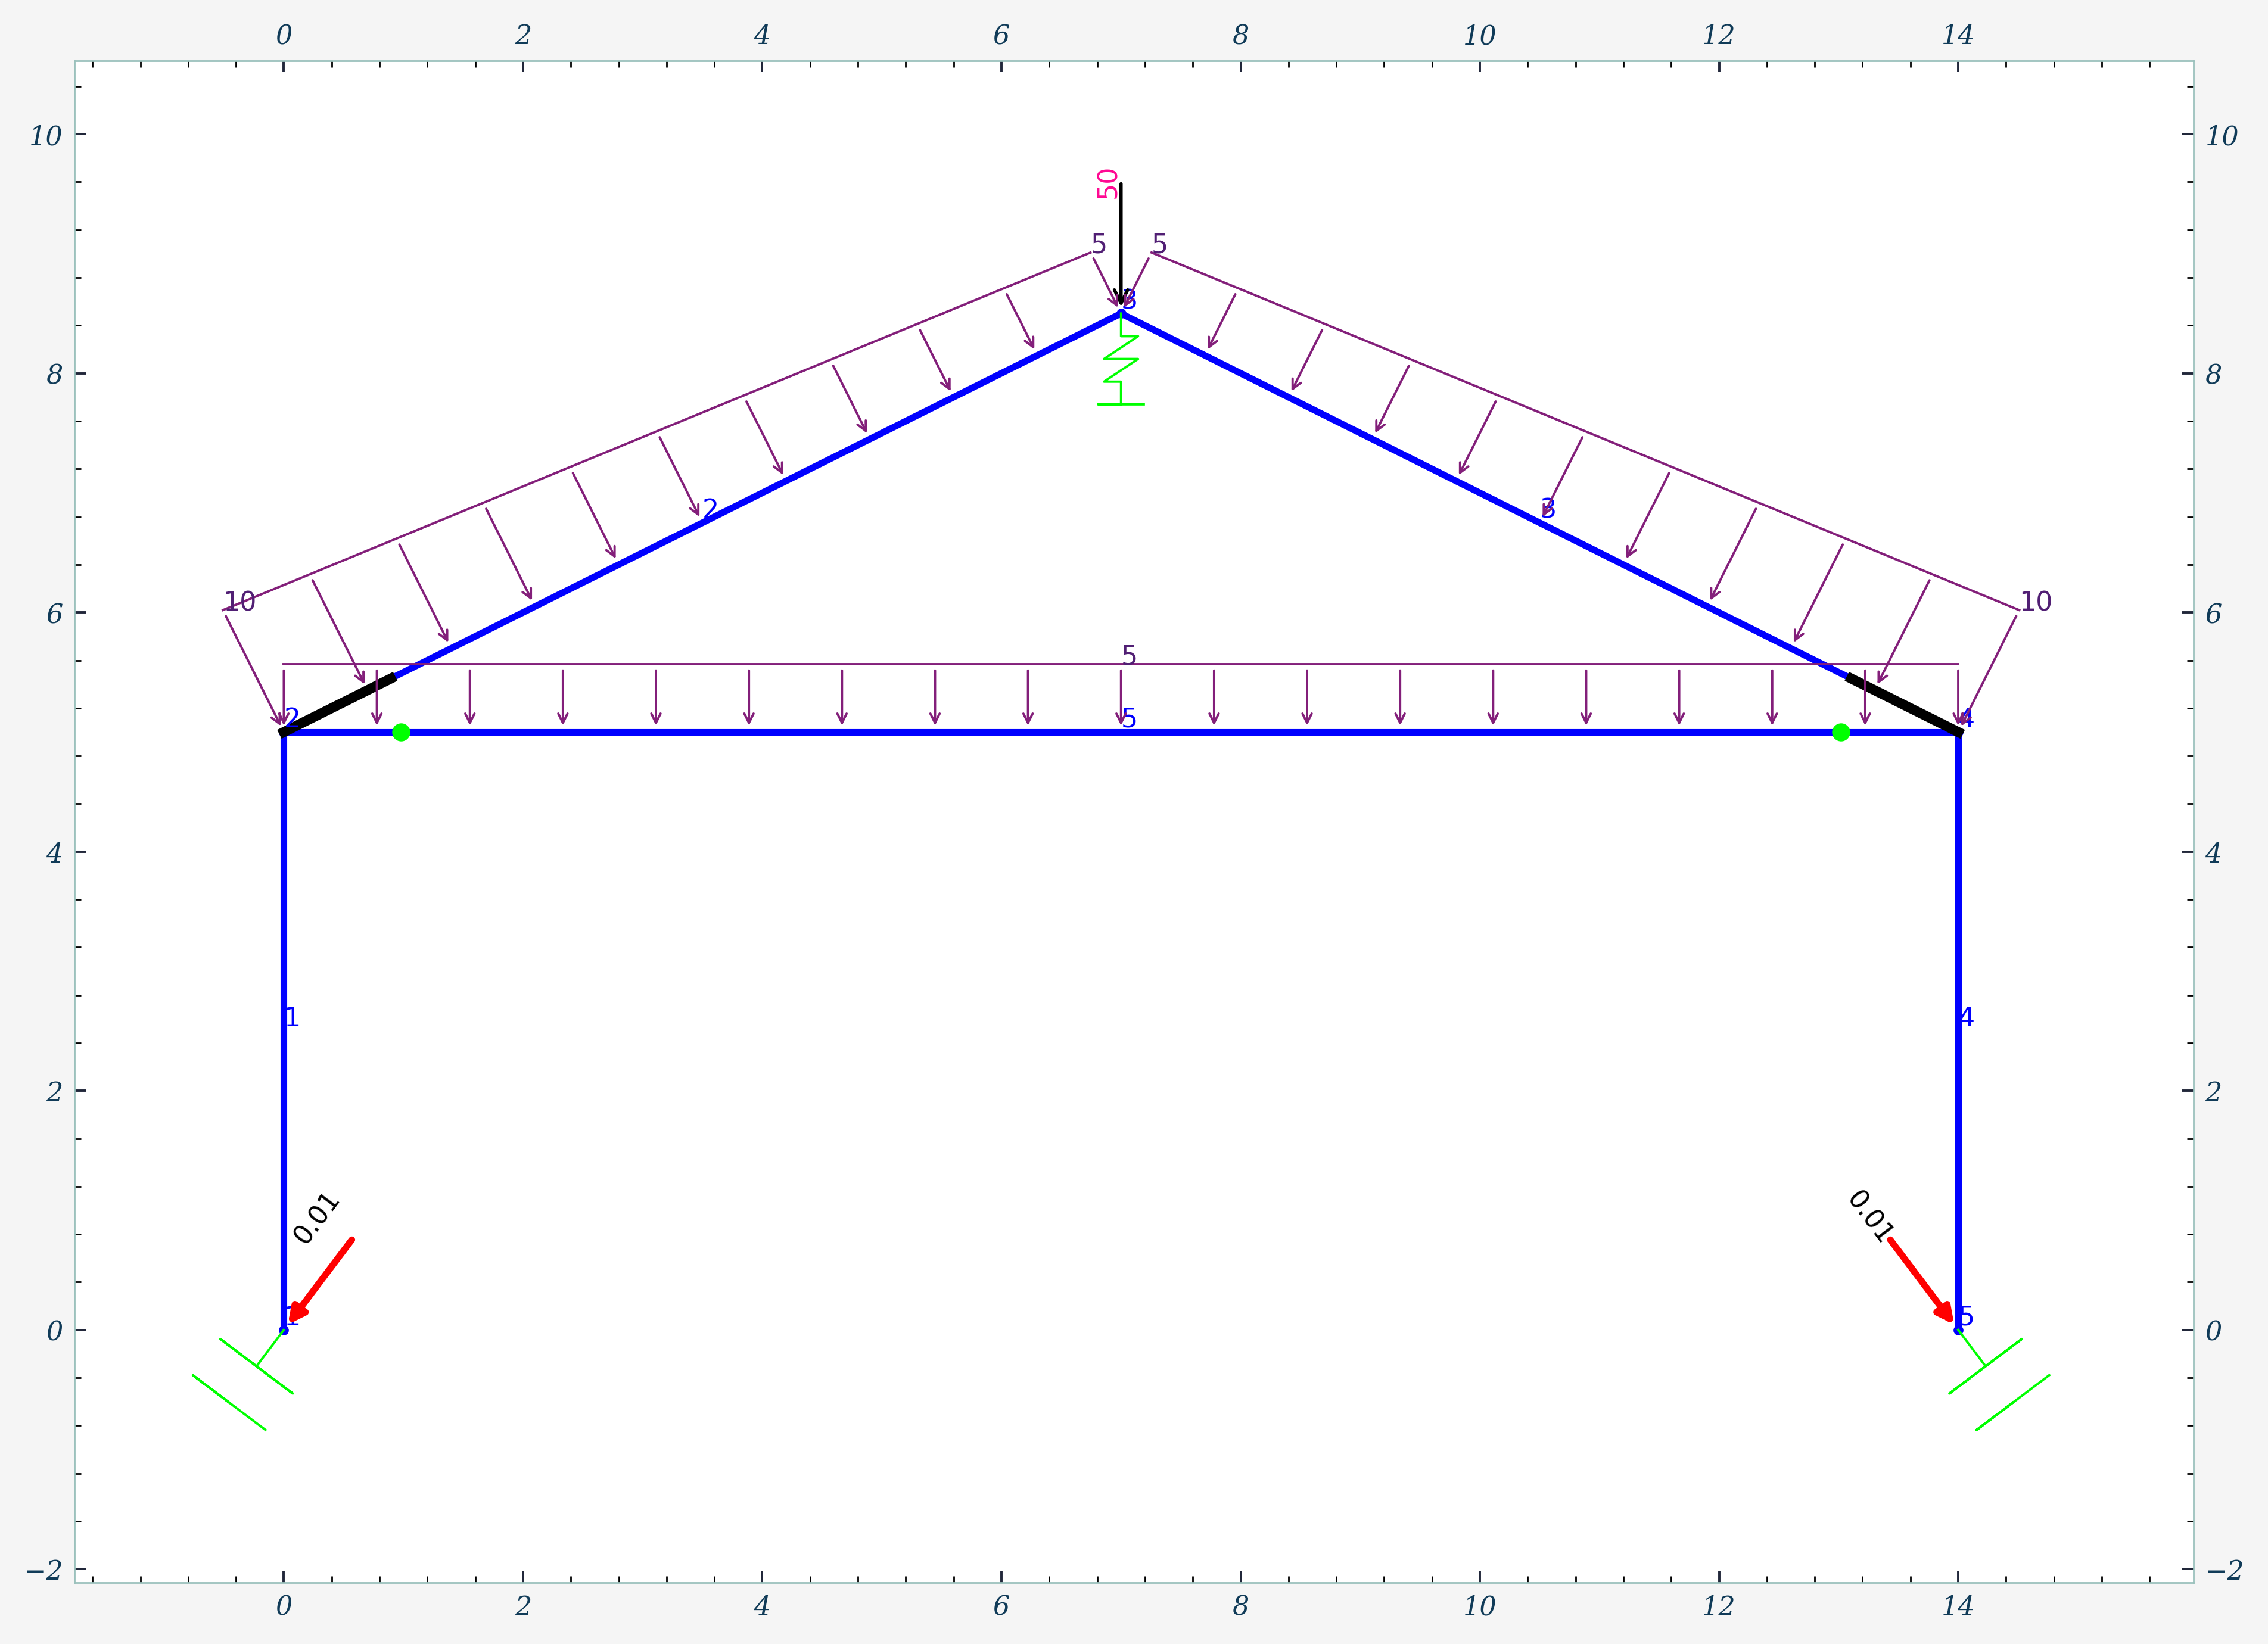
\includegraphics[width=1\textwidth]{img/modelo.png}
\subsection{Materiales}
\subsection{Secciones}
\subsection{Modificadores de sección}
\subsection{Nodos}
\subsection{Elementos}
\subsection{Asignación de Cargas}
\subsection{Asignación de Desplazamientos}
\subsection{Suportes}
\subsection{Ejes Locales en Nudos}
\subsection{Apoyos Elásticos}
\subsection{Brazos Rígidos}
\subsection{Liberaciones de Esfuerzos en los Extremos}



\section{Resultados}
\subsection{Cuadro General de Resultados}
\subsection{Diagrama de Fuerzas Axiales}
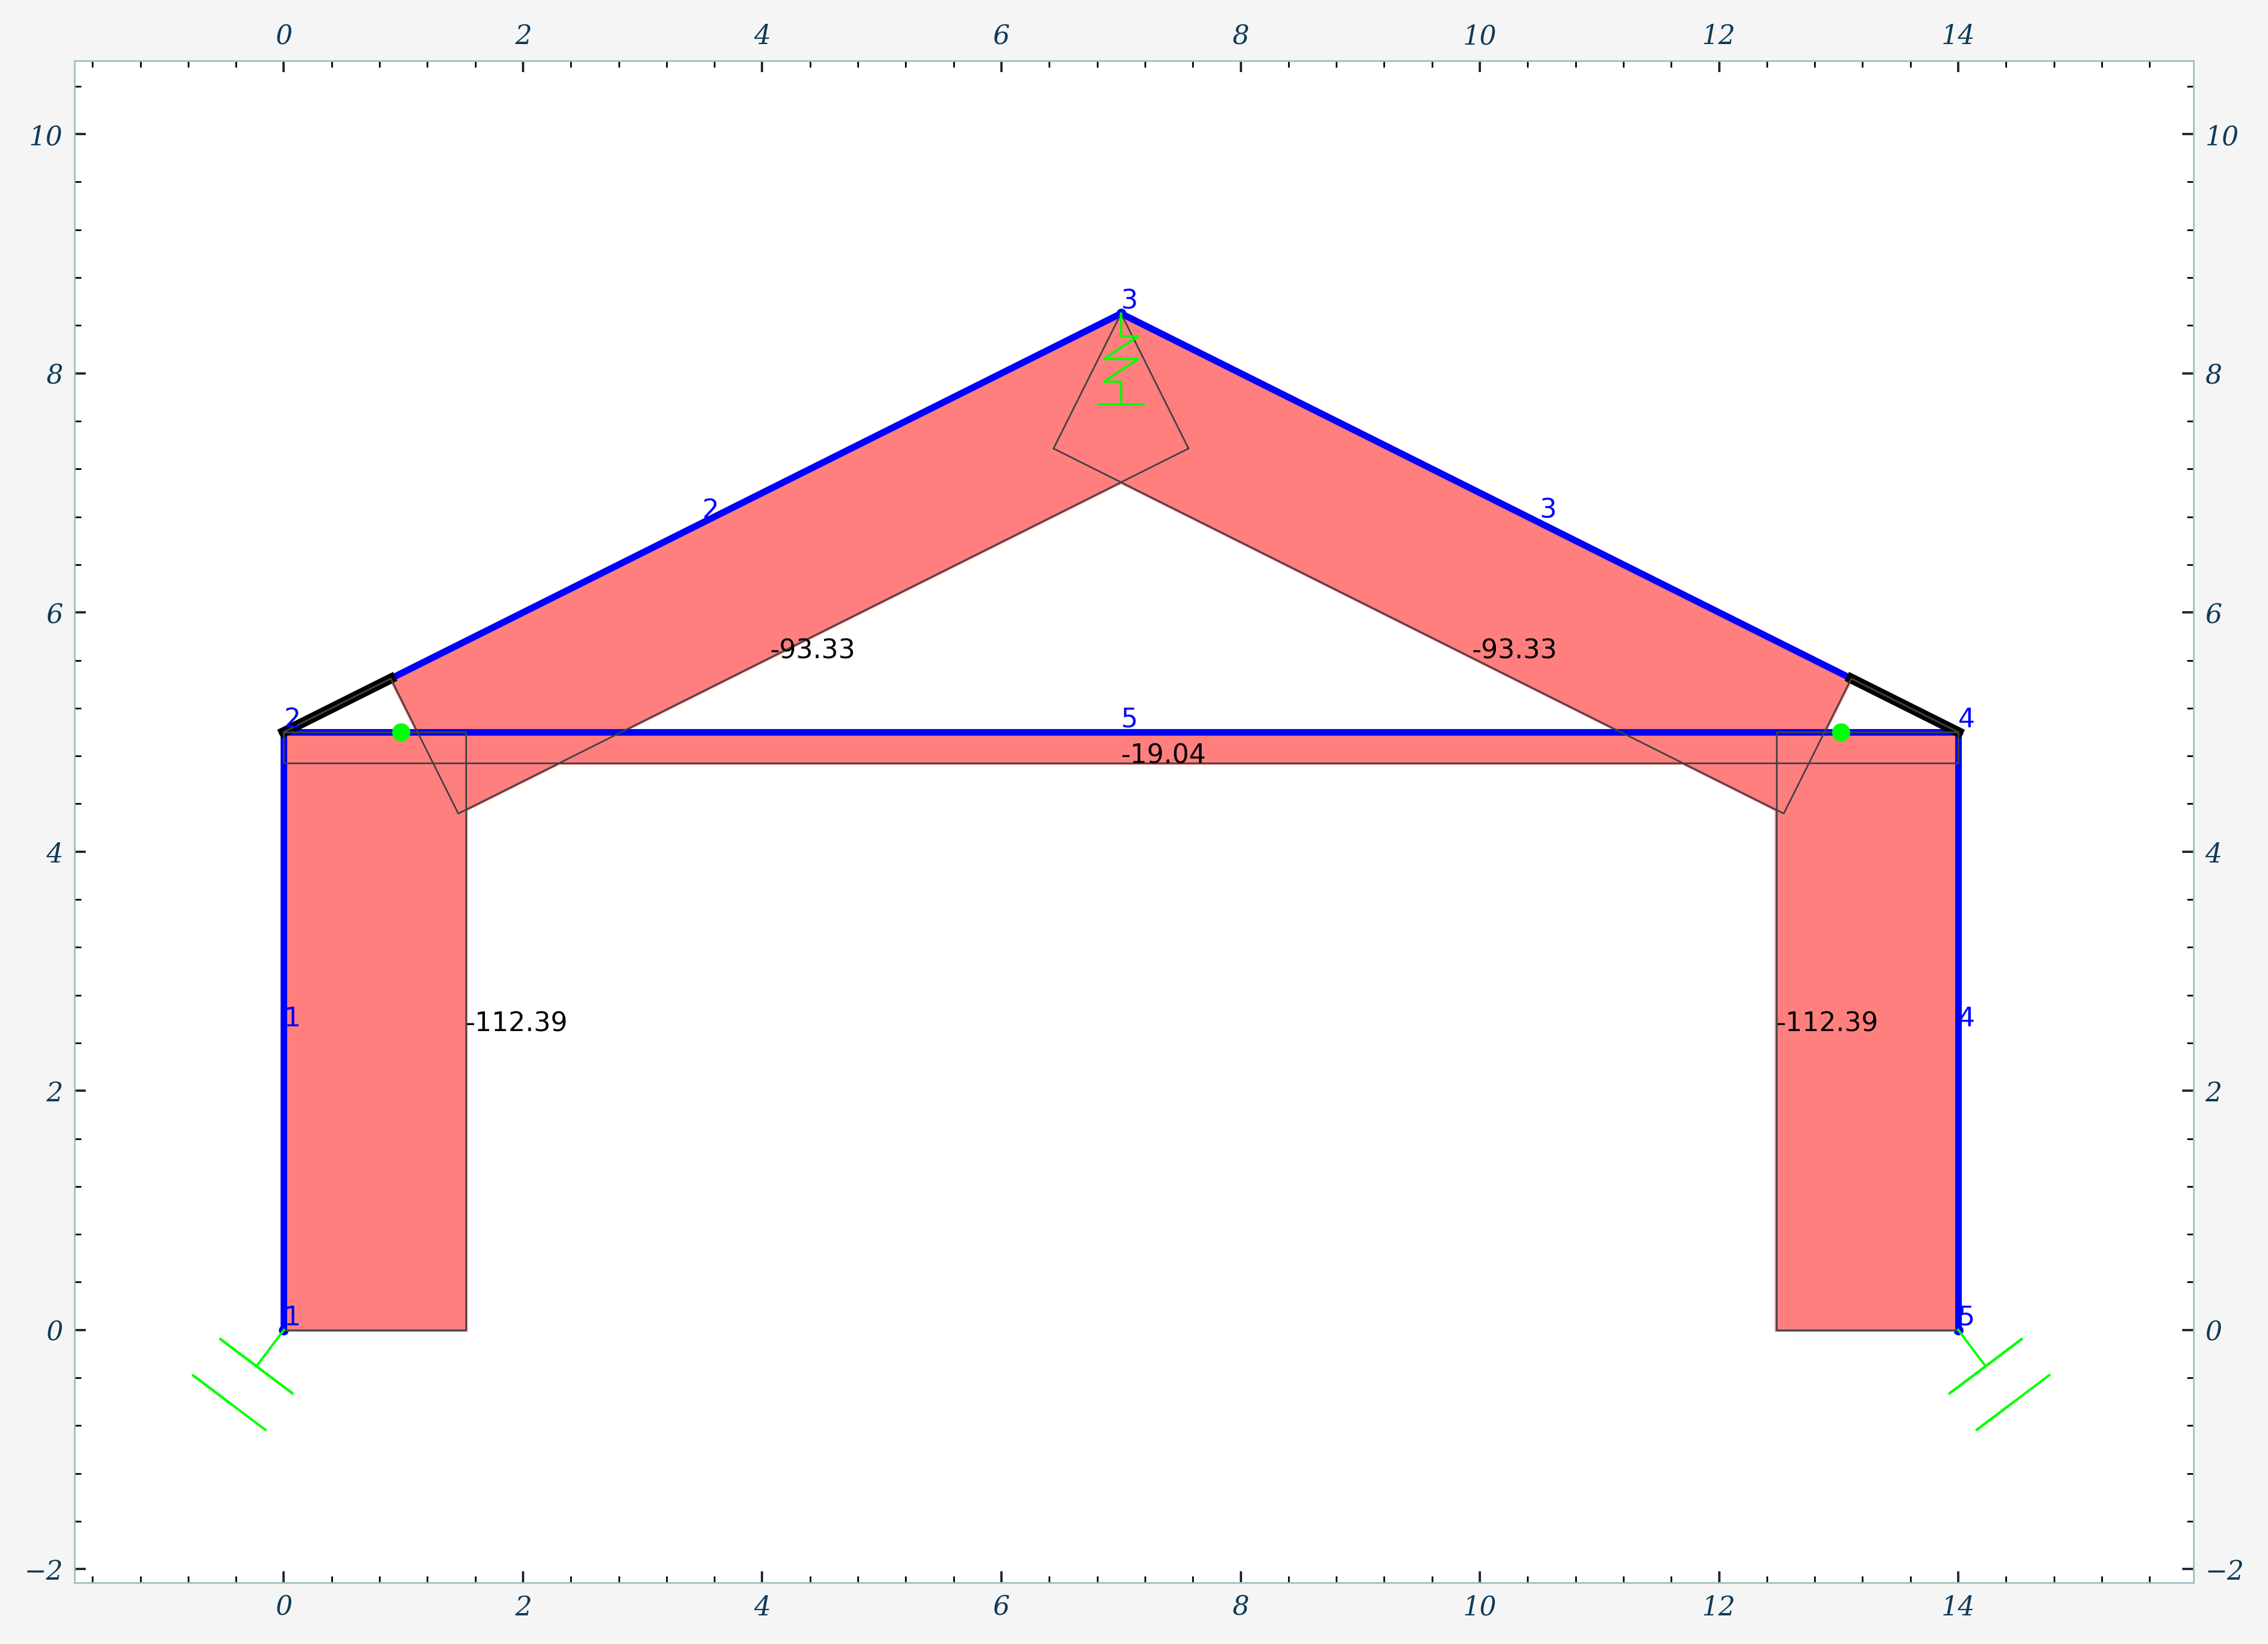
\includegraphics[width=1\textwidth]{img/diag_axiales.png}

\subsection{Diagrama de Fuerzas Cortantes}
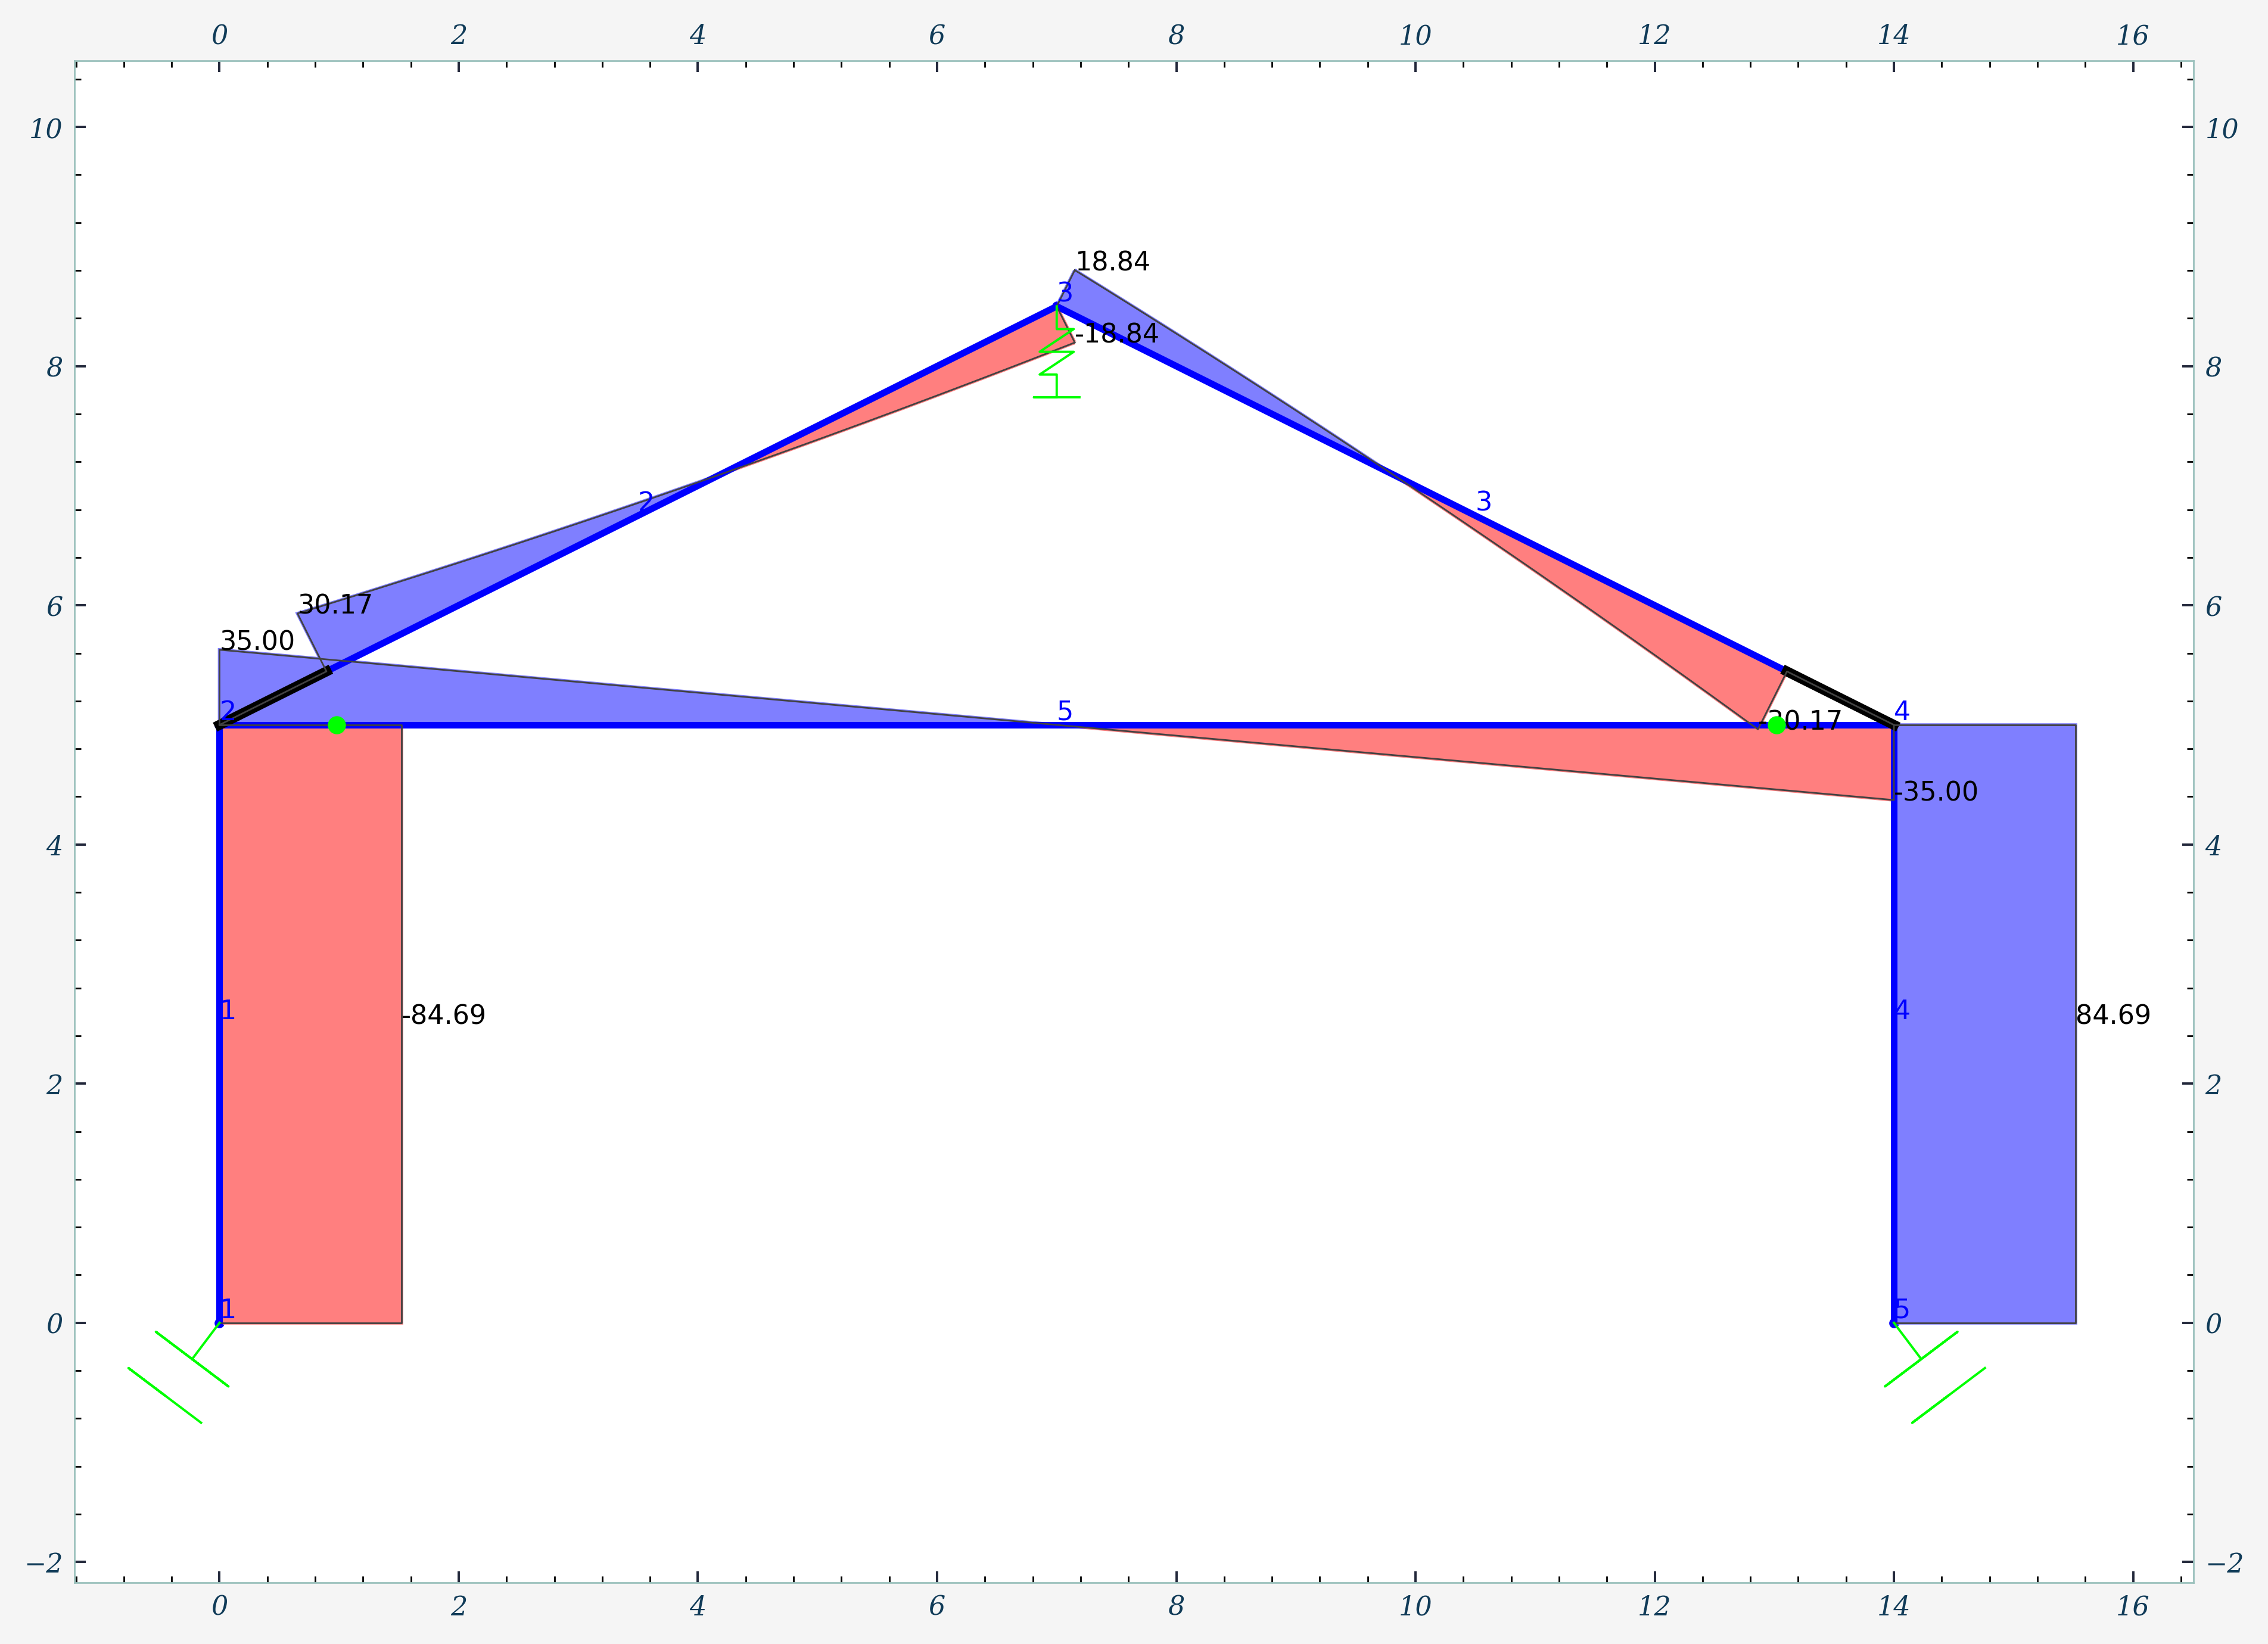
\includegraphics[width=1\textwidth]{img/diag_cortantes.png}

\subsection{Diagrama de Fuerzas Momentos}
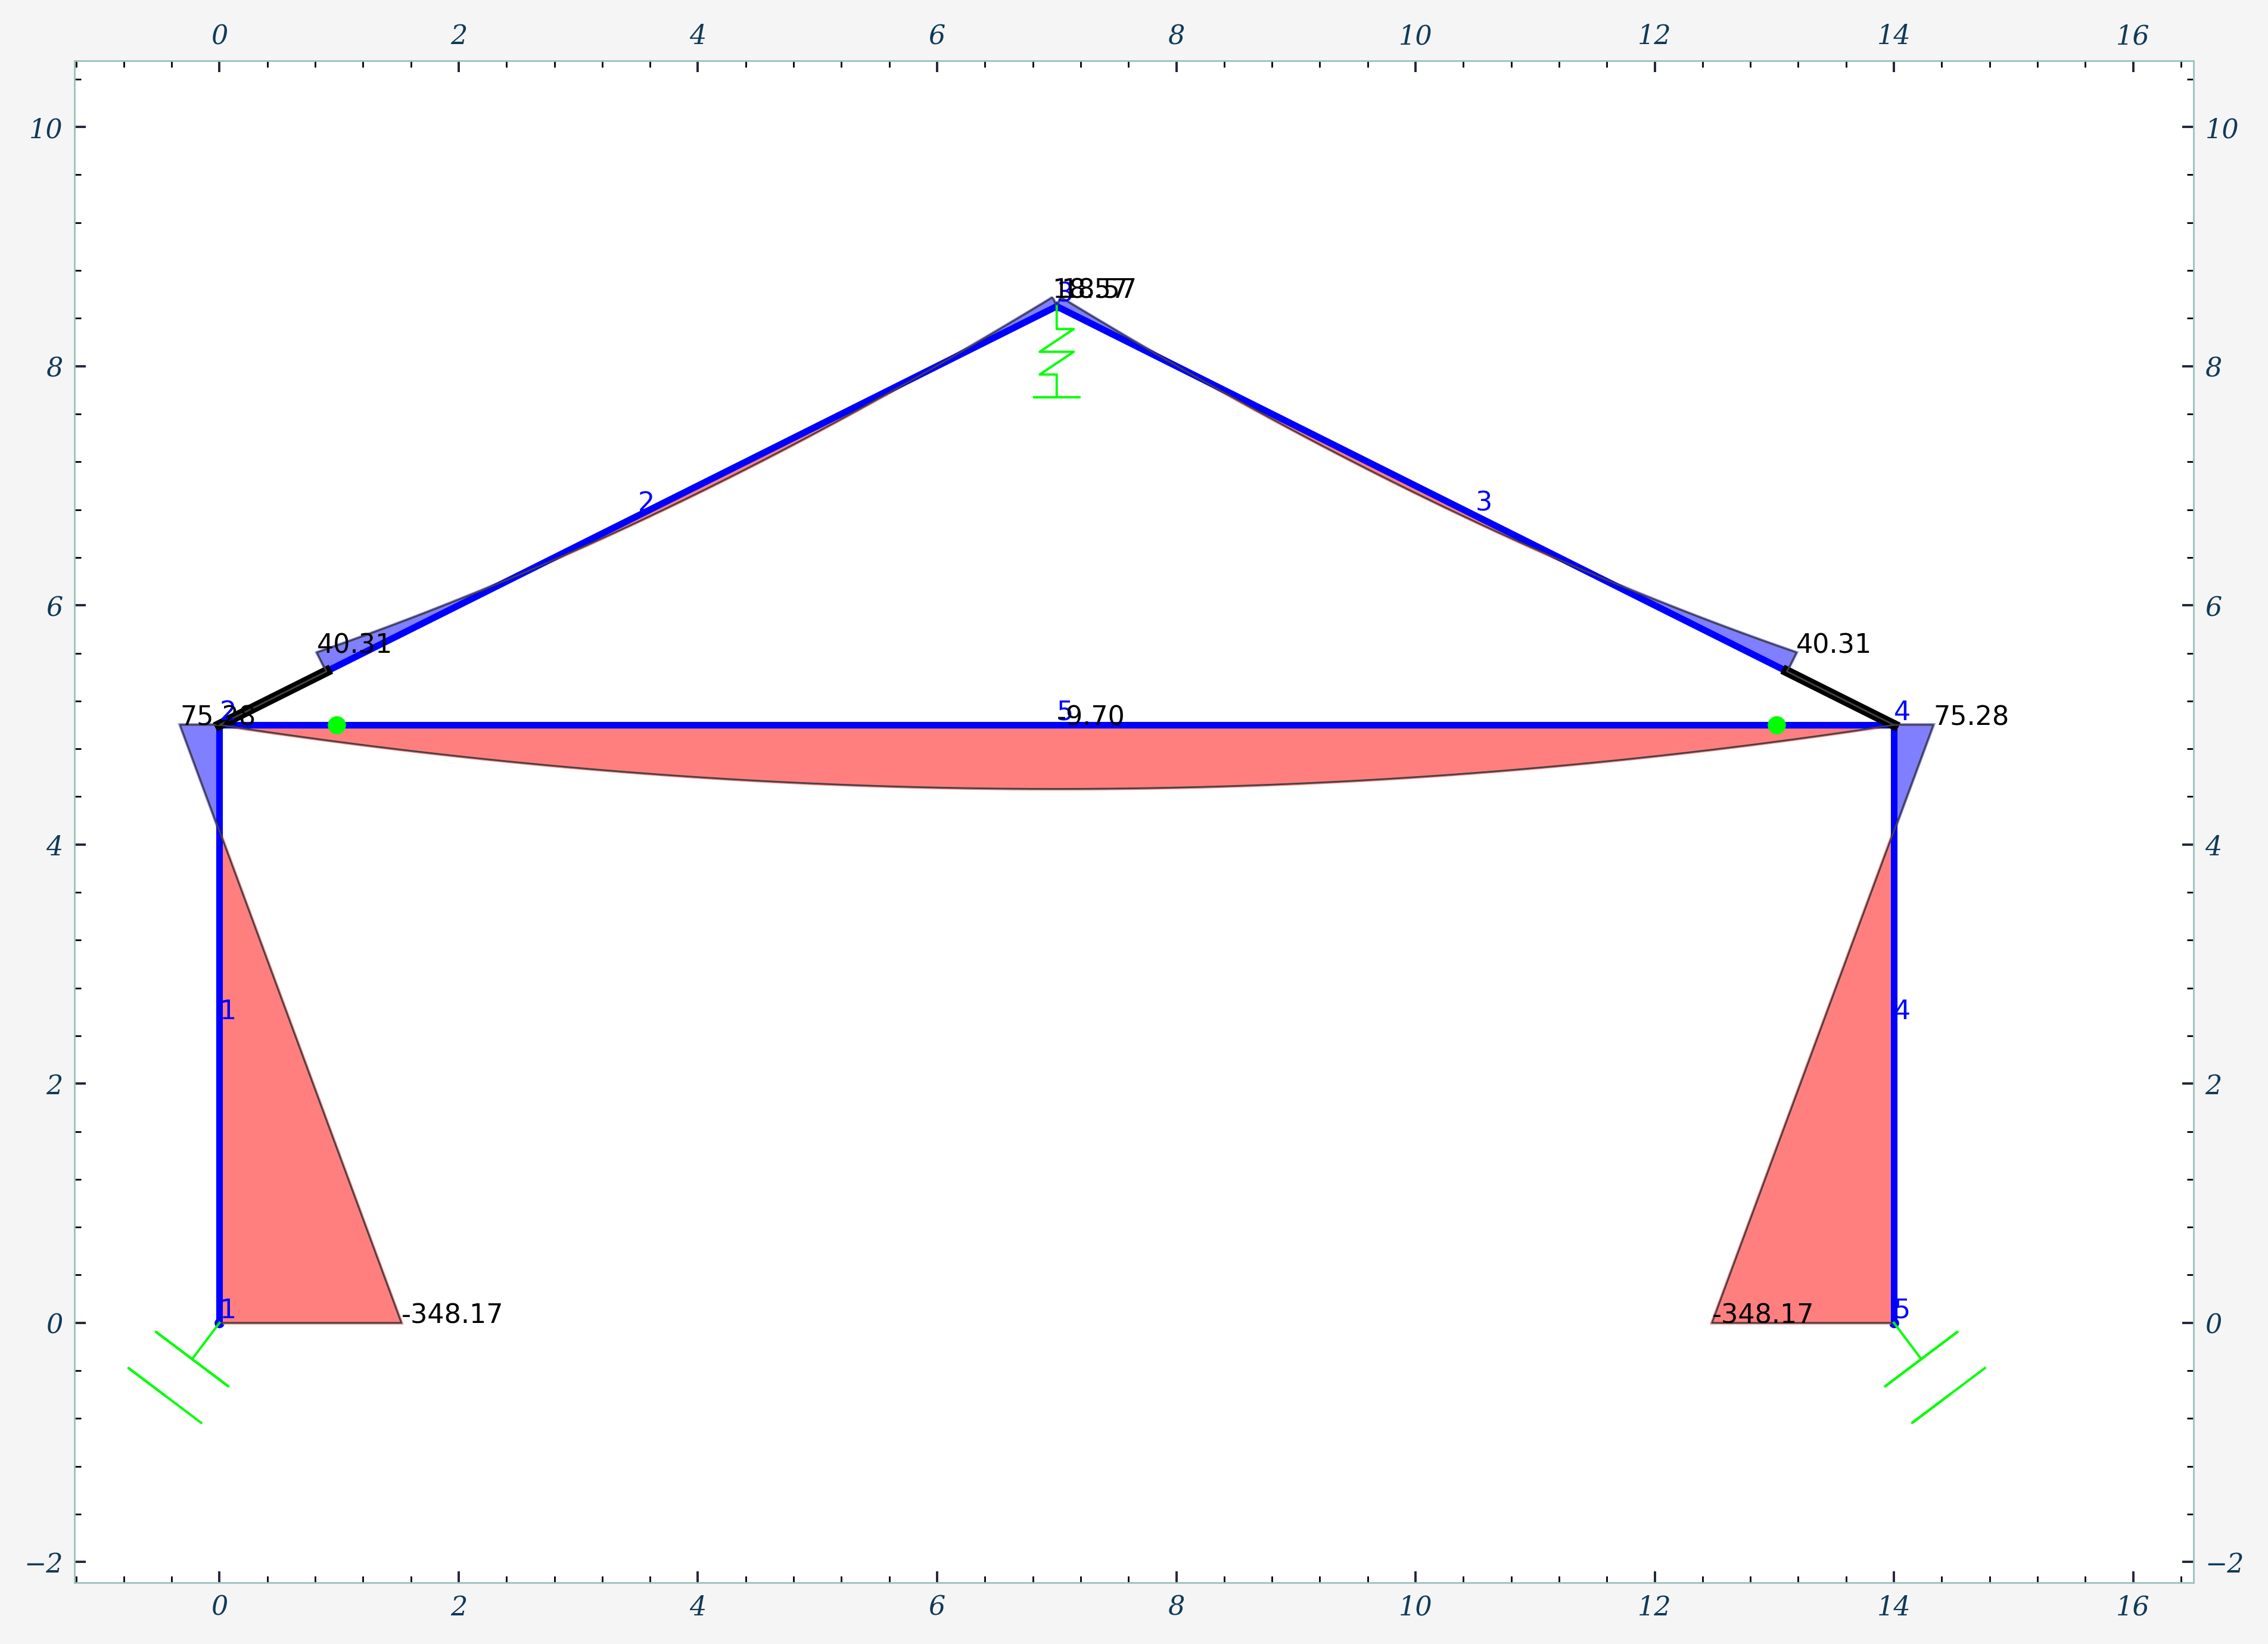
\includegraphics[width=1\textwidth]{img/diag_momentos.png}

\subsection{Deformada Rígida}
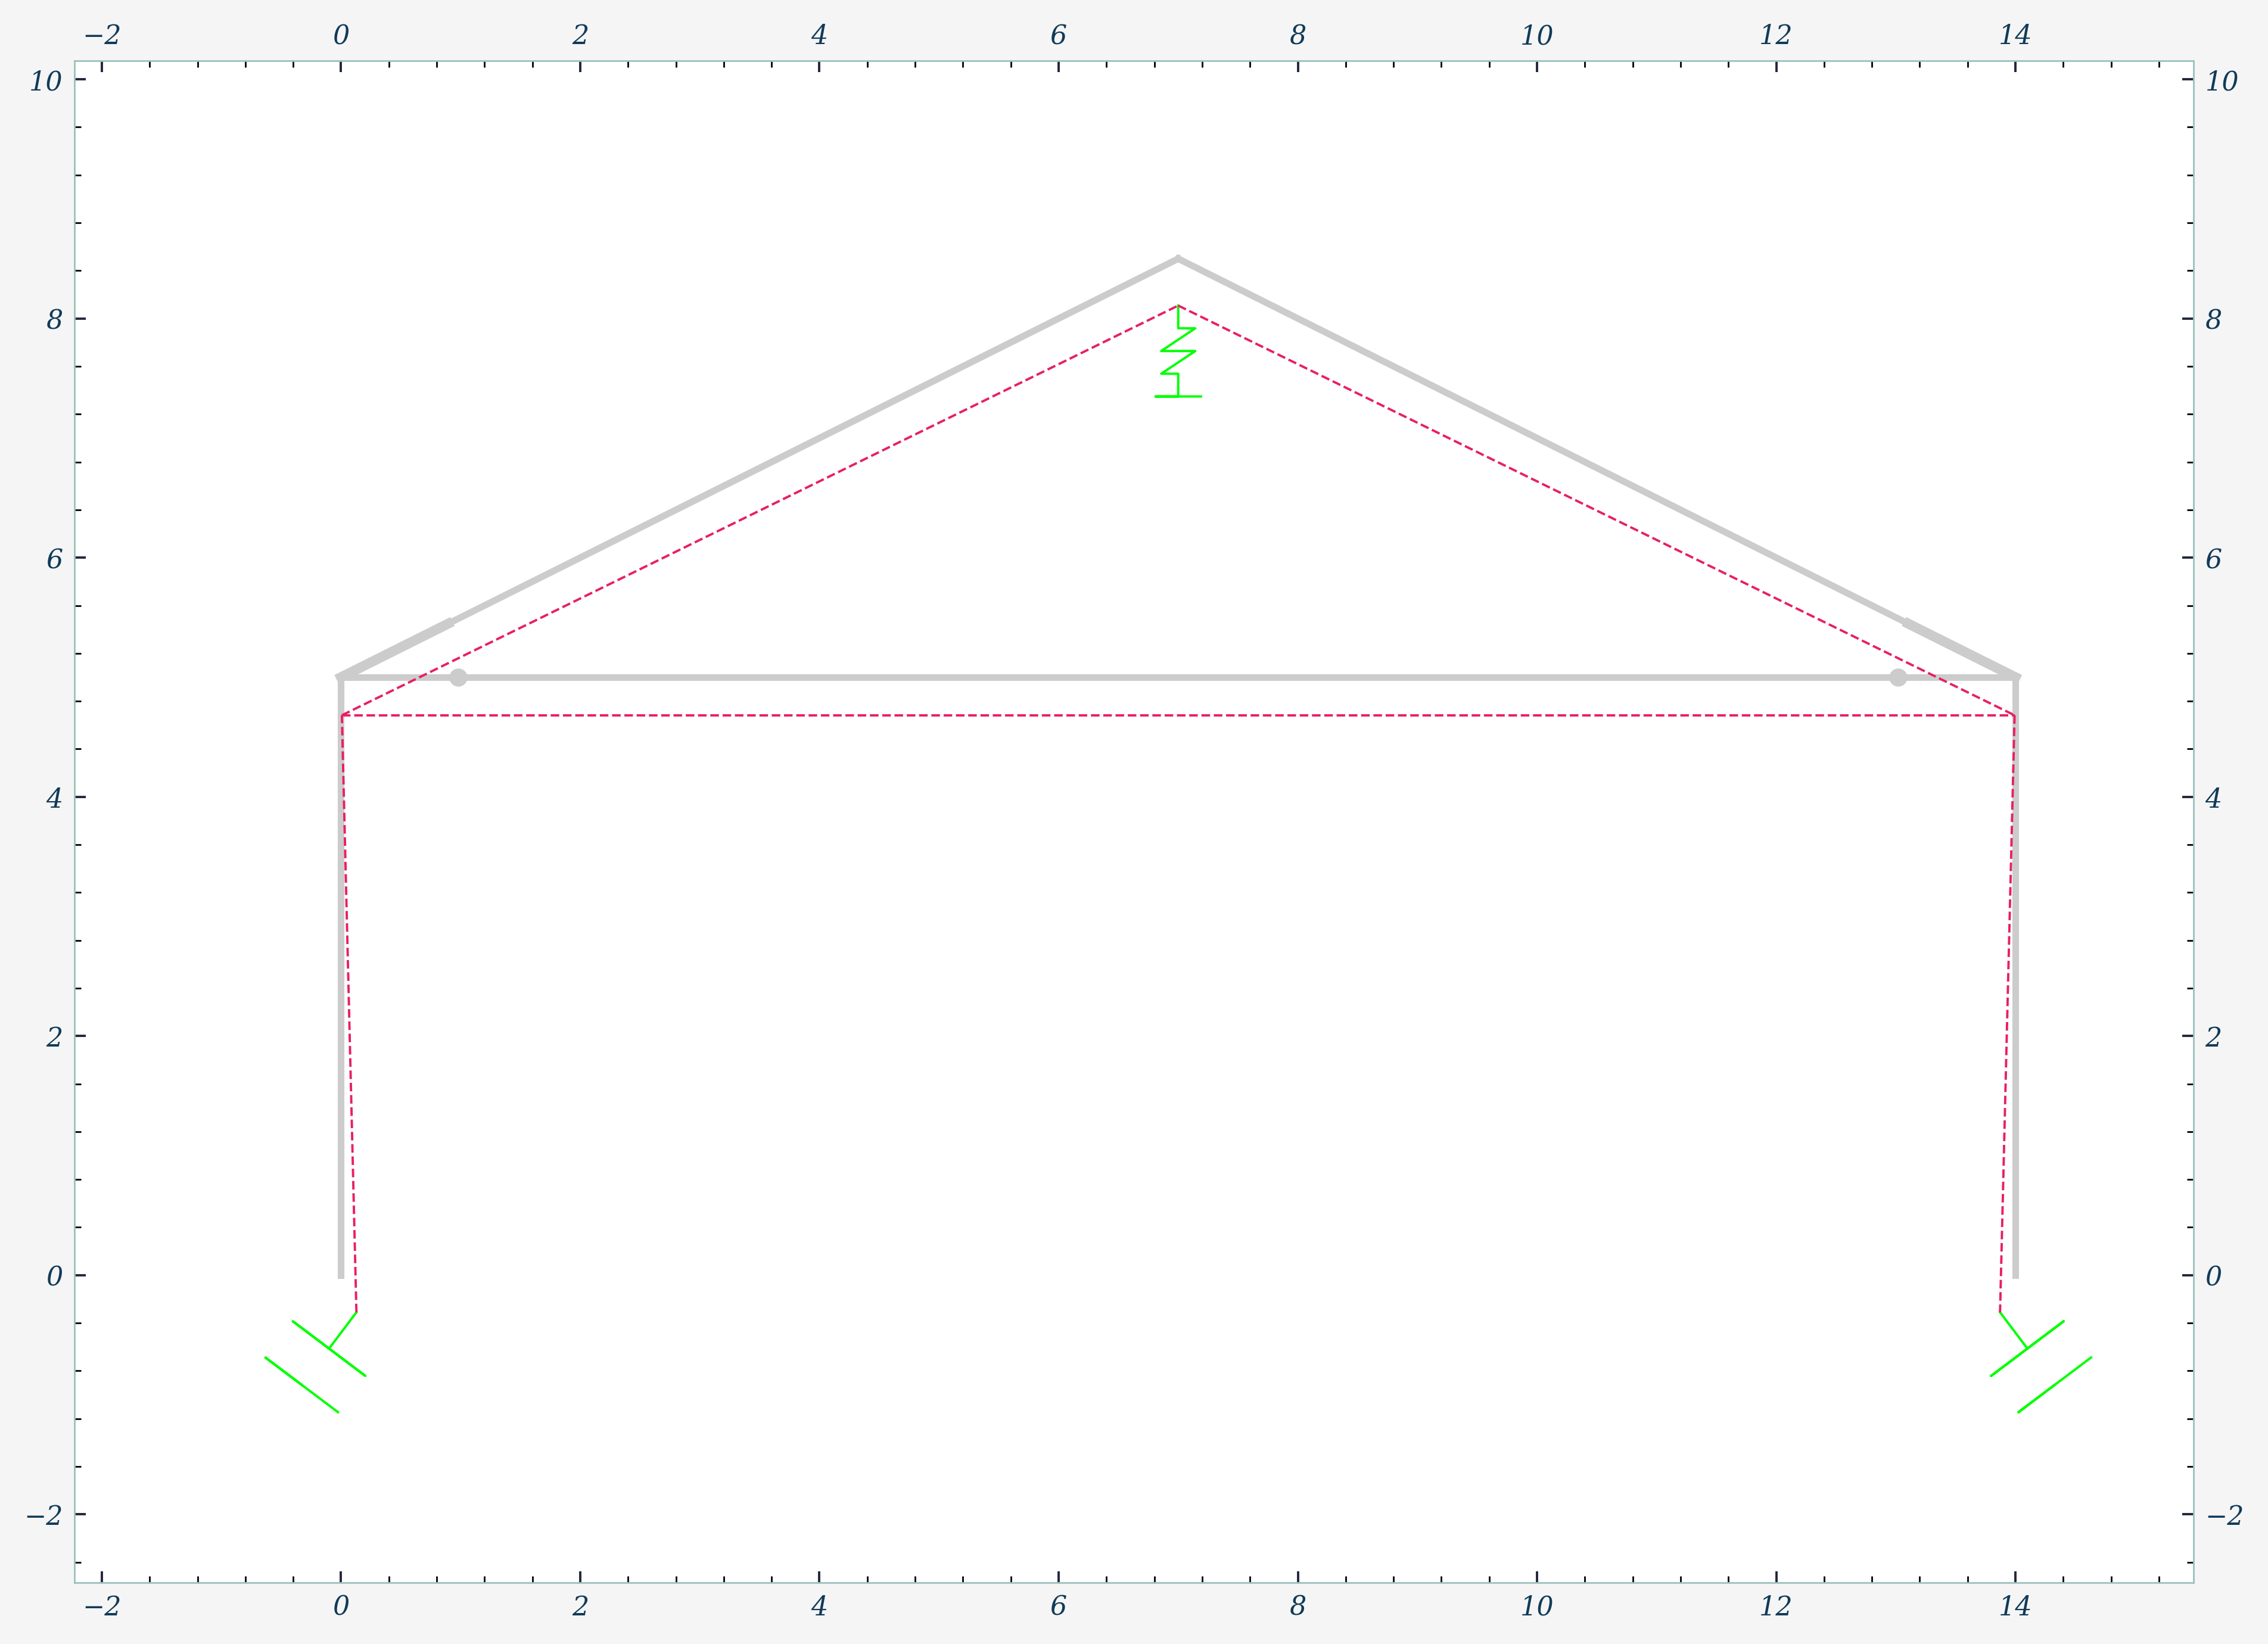
\includegraphics[width=1\textwidth]{img/deforma_rigida.png}

\subsection{Deformada de la Estructura}
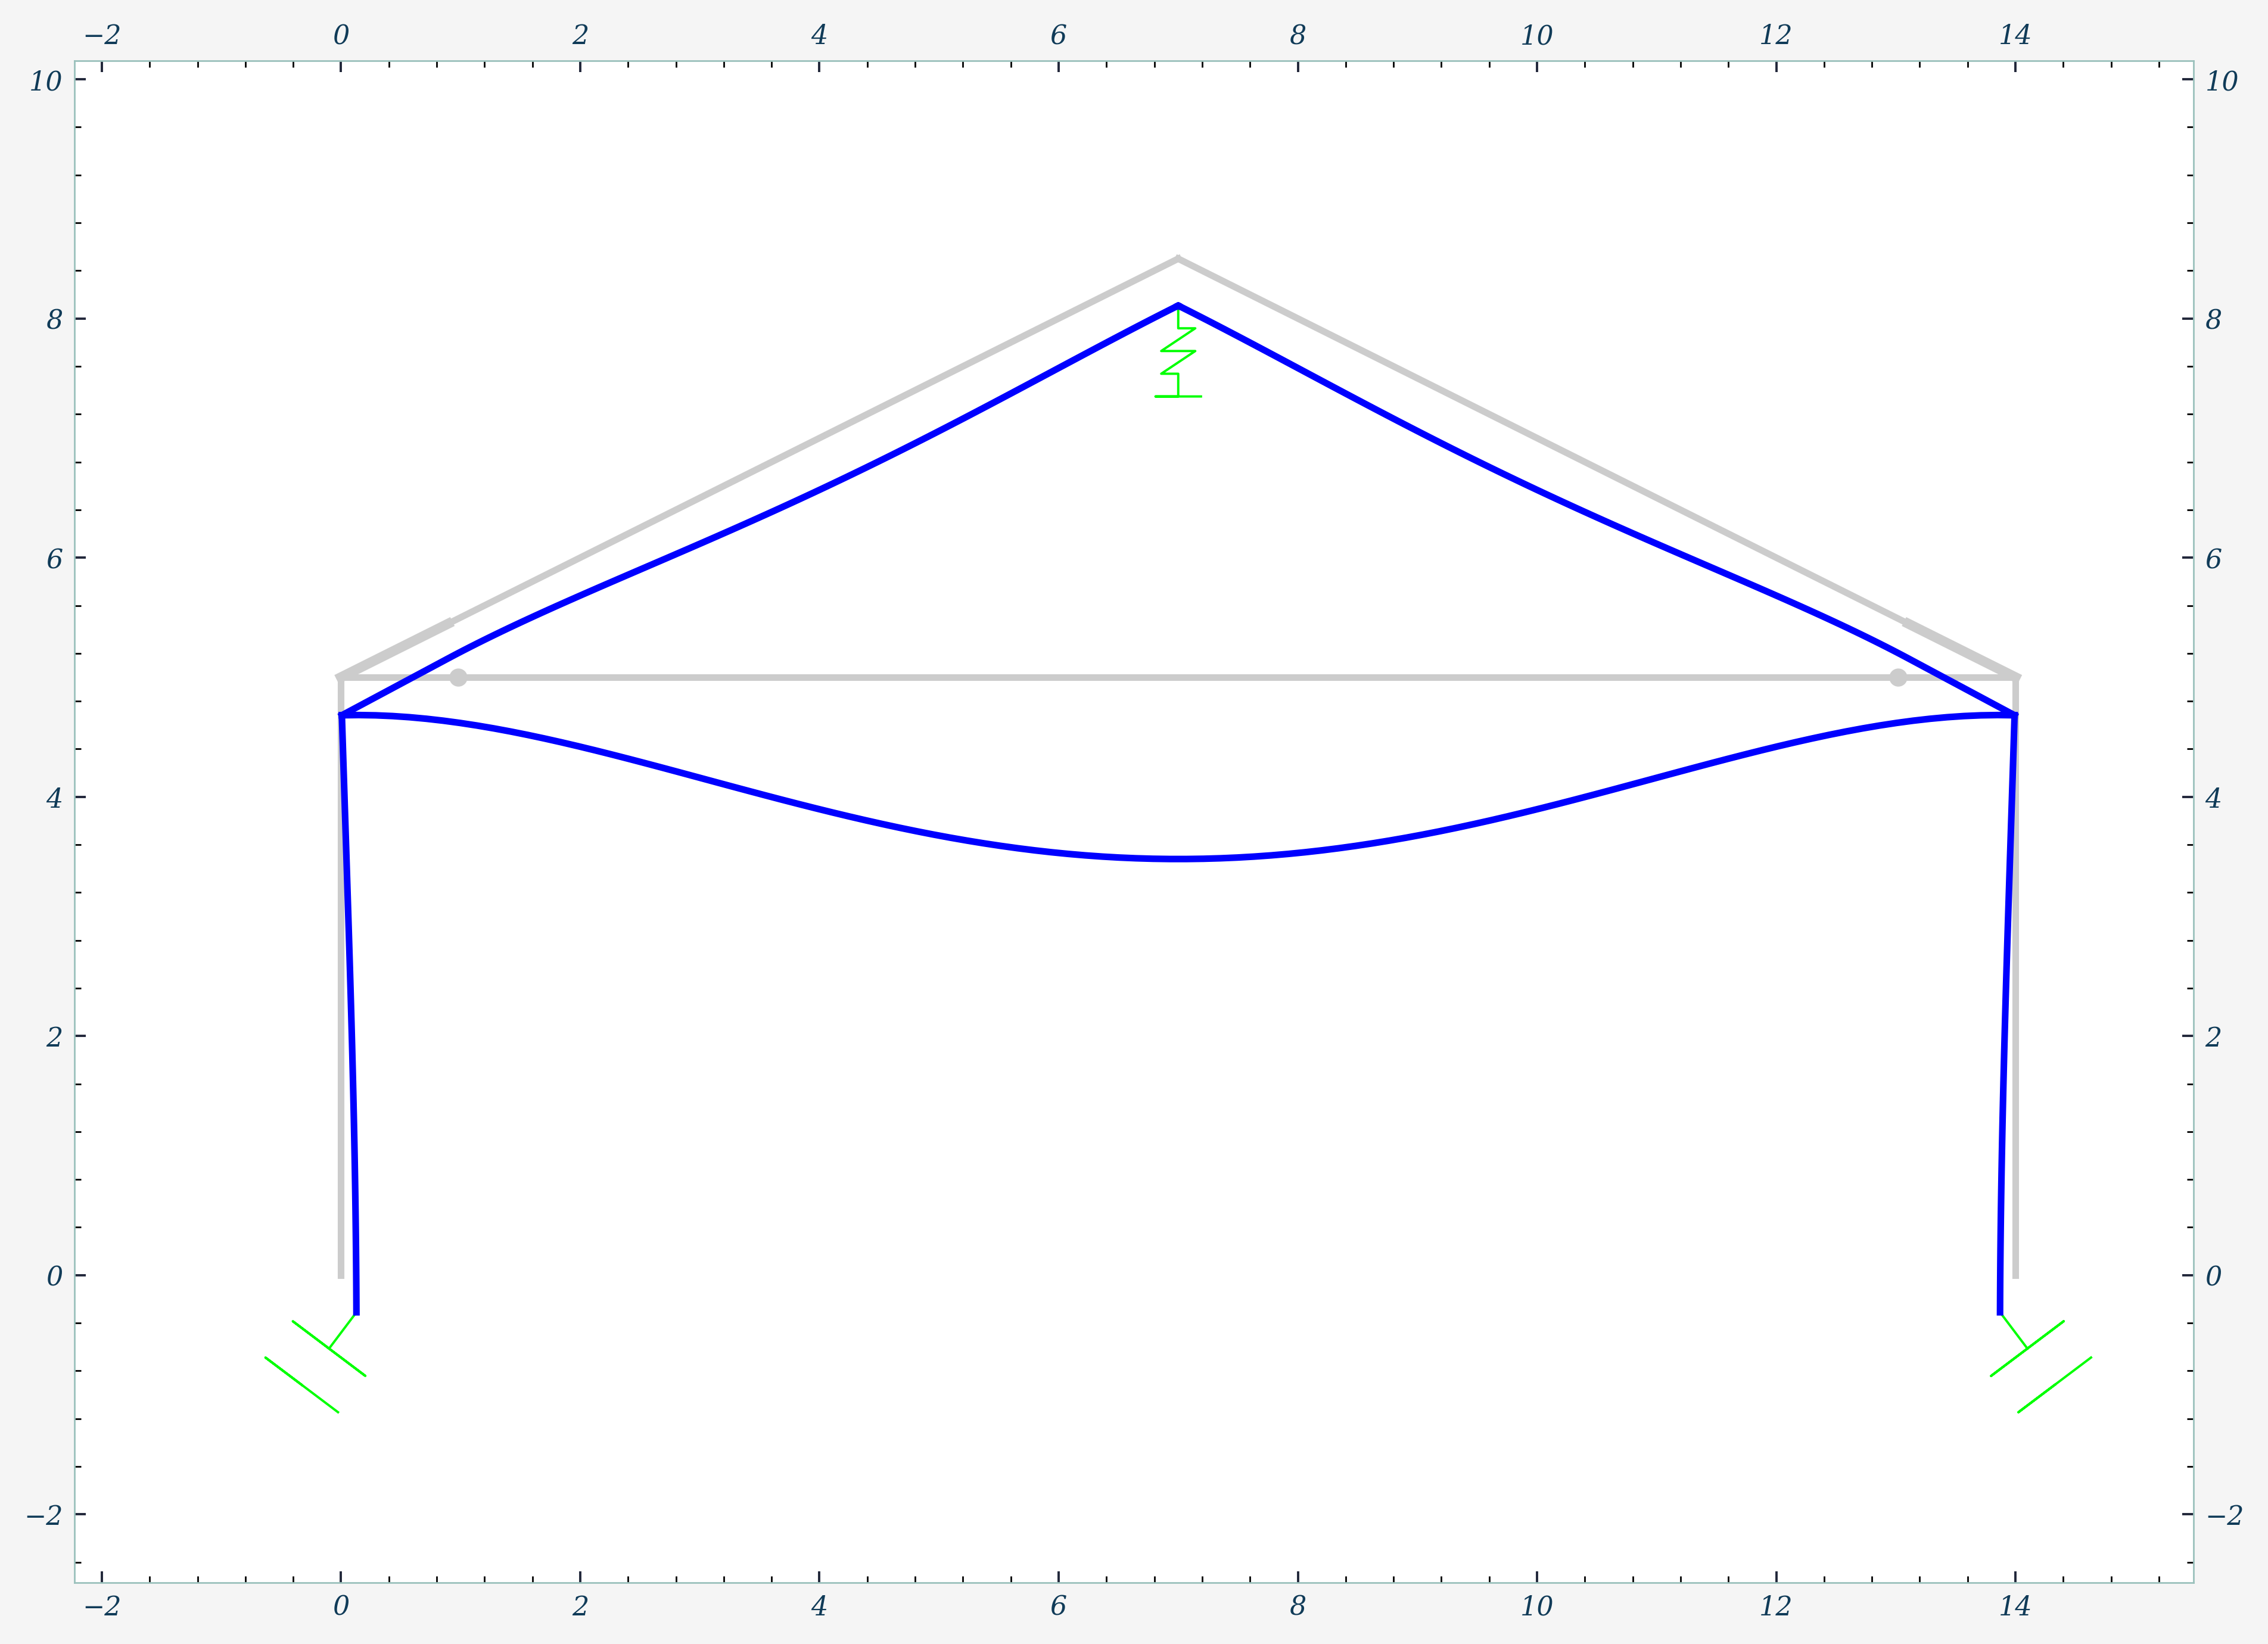
\includegraphics[width=1\textwidth]{img/deformada.png}

\subsection{Gráfico de Reacciones}
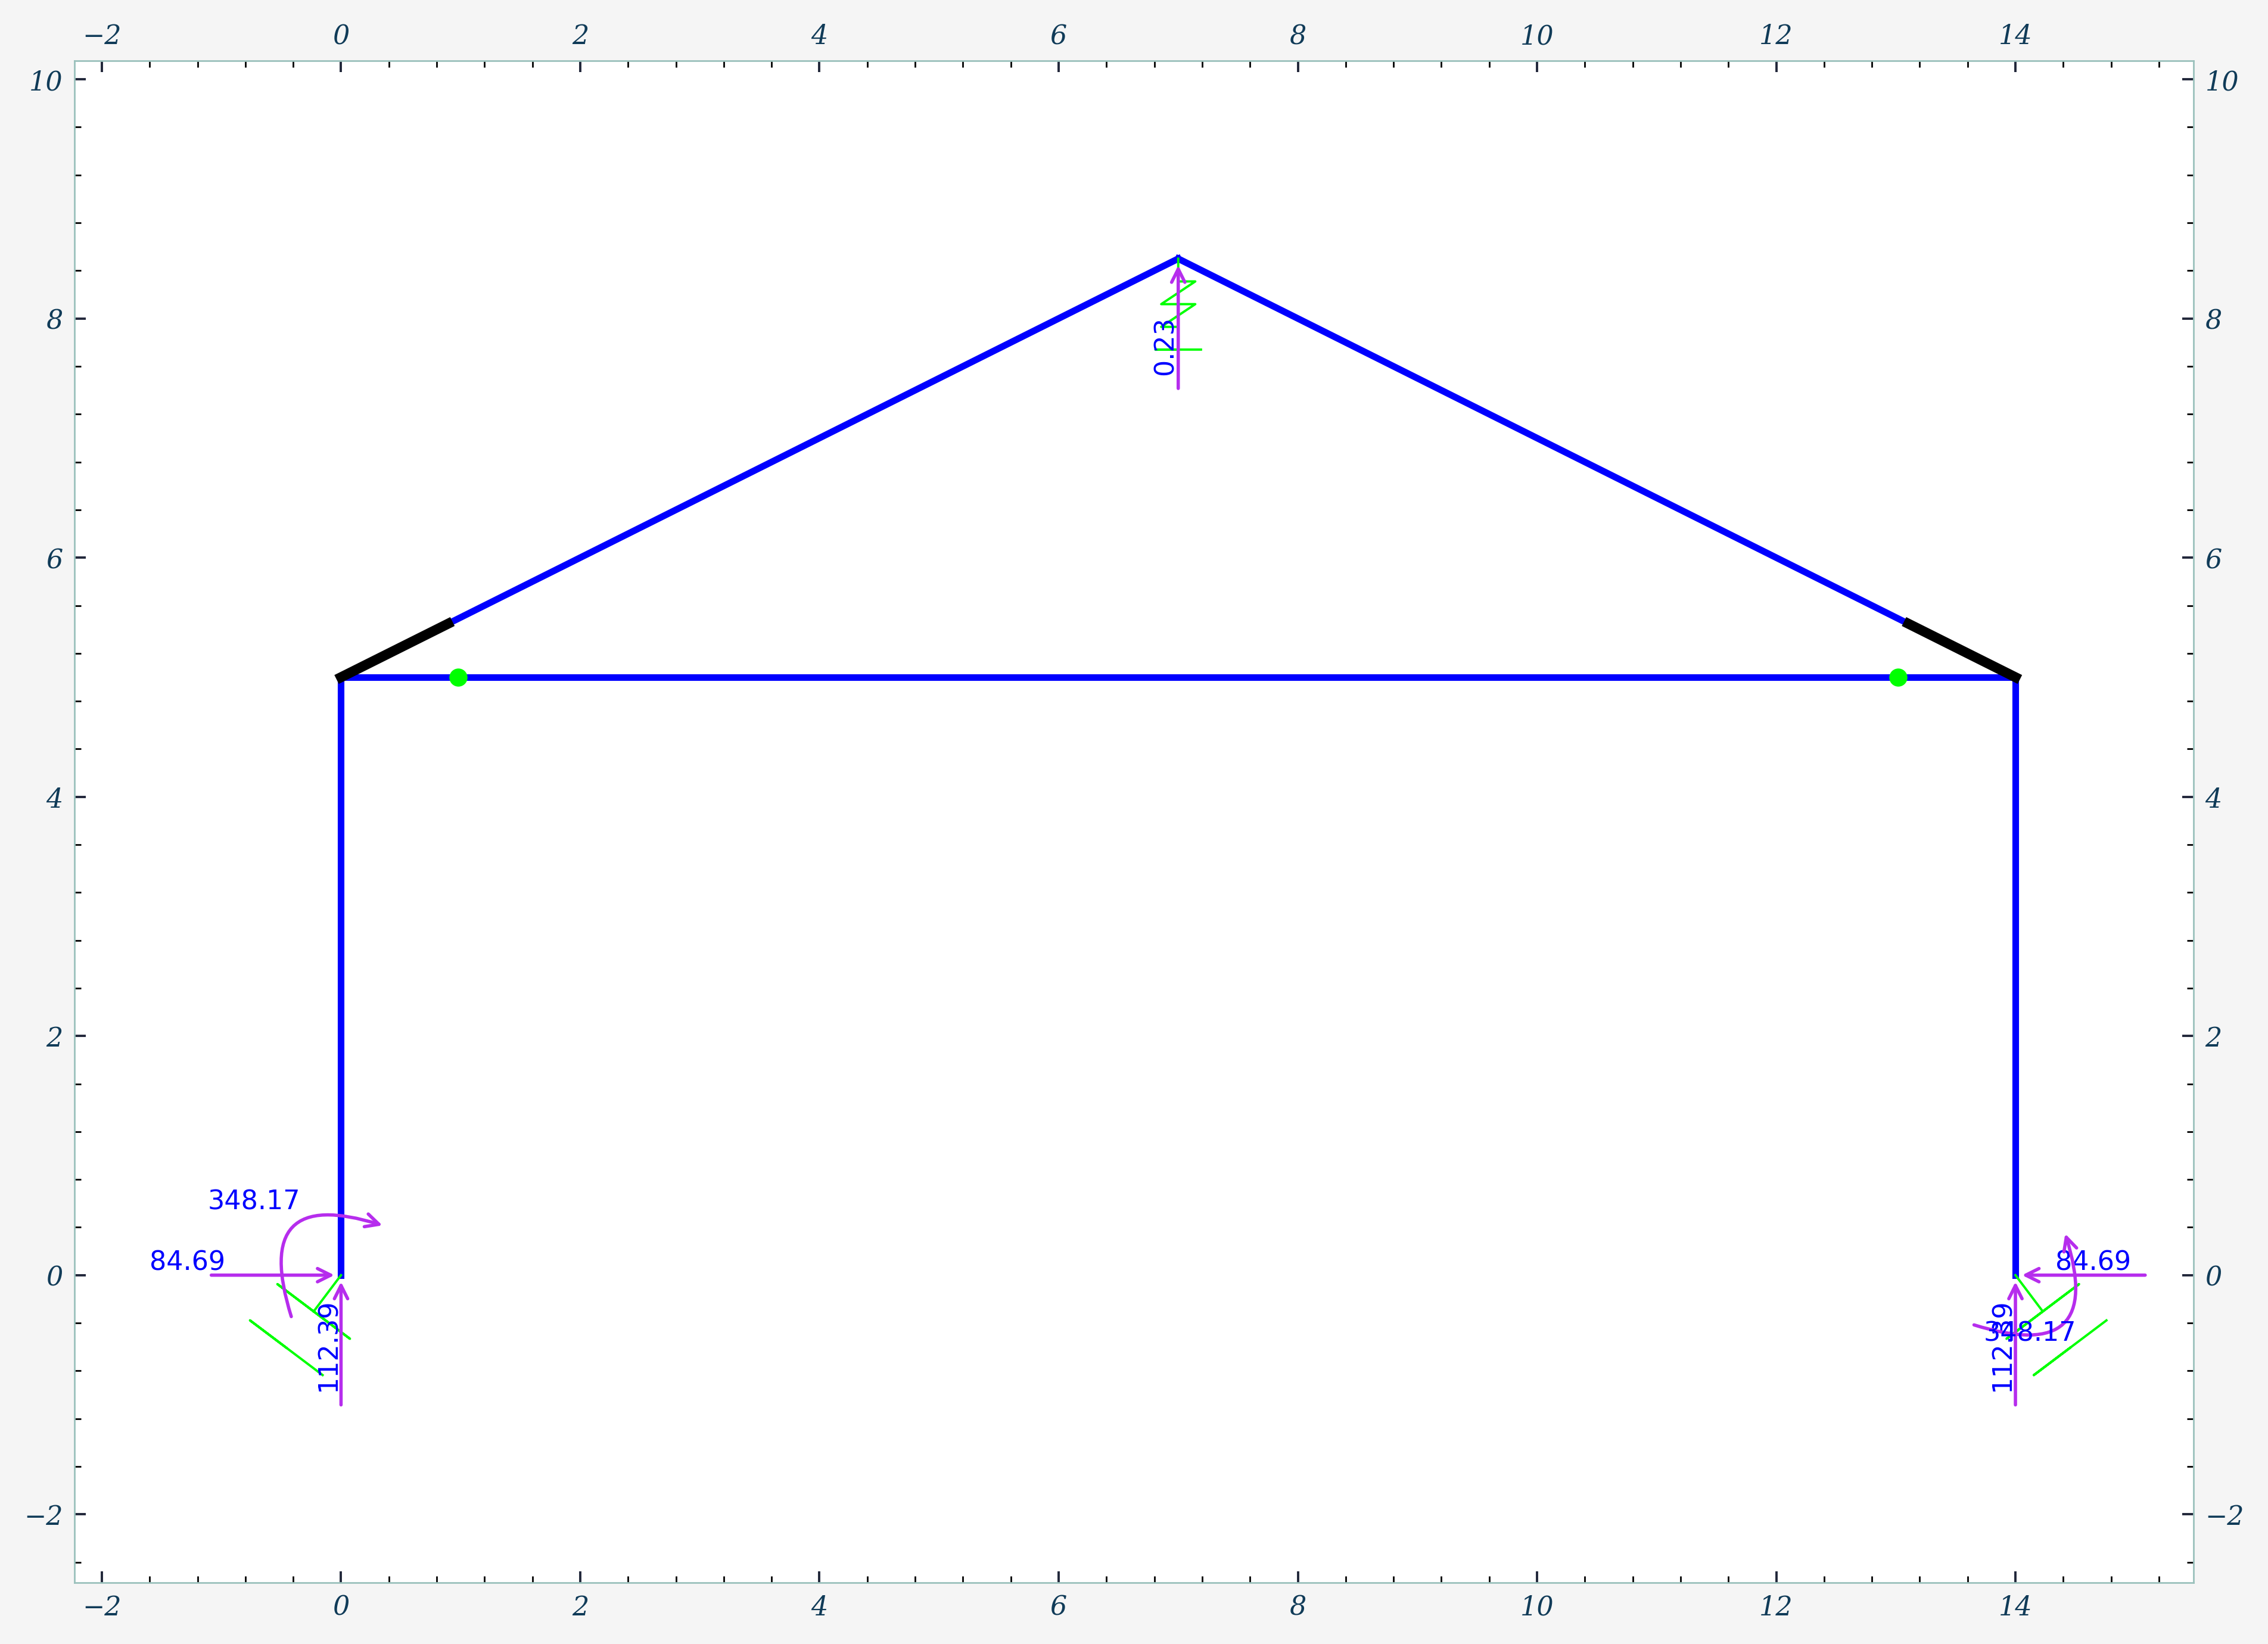
\includegraphics[width=1\textwidth]{img/reacciones.png}

  % Capítulo 1


% Fin del documento
\end{document}
